\documentclass[12pt,oneside]{book}
\usepackage[a4paper,margin=2.5cm,headheight=25pt]{geometry}
\usepackage[T1]{fontenc}
\usepackage[utf8]{inputenc}
\usepackage[french]{babel}
\usepackage{lmodern}
\usepackage{microtype}
\usepackage{amsmath,amssymb}
\usepackage{graphicx}
\usepackage{booktabs,longtable,tabularx,array,multirow}
\usepackage{float}
\usepackage{caption}
\usepackage{xcolor}
\usepackage{enumitem}
\usepackage{fancyhdr}
\usepackage{titlesec}
\usepackage{tcolorbox}
\usepackage{lastpage}
\usepackage{hyperref}
\usepackage{bookmark}
\usepackage{csquotes}
\usepackage{tikz}
\usetikzlibrary{positioning}
\usepackage{listings}
\usepackage{textcomp}
\usepackage{placeins}
\usepackage[backend=biber,style=authoryear,sorting=nyt]{biblatex}
\addbibresource{references.bib}
\definecolor{navy}{HTML}{12304A}
\definecolor{gold}{HTML}{B8903A}
\definecolor{lightnavy}{HTML}{EAF1F5}
\definecolor{darkgray}{HTML}{3F4A52}
\hypersetup{colorlinks=true,linkcolor=navy,citecolor=navy,urlcolor=navy,pdftitle={Conception d'une solution décisionnelle pour MetroPT-3},pdfauthor={Saad Sahraoui; Hassan El Hajjam; Yassine Saddane}}
\graphicspath{{figures/dashboards/}{figures/architecture/}{assets/logos/}}
\setlength{\parindent}{0pt}
\setlength{\parskip}{0.55em}
\renewcommand{\arraystretch}{1.2}
\setlist[itemize]{leftmargin=*,itemsep=2pt}
\setlist[enumerate]{leftmargin=*,itemsep=2pt}
\titleformat{\chapter}[display]{\bfseries\color{navy}}{\fontsize{15}{18}\selectfont\chaptername\ \thechapter}{8pt}{\Huge}
\titlespacing*{\chapter}{0pt}{-10pt}{24pt}
\titleformat{\section}{\Large\bfseries\color{navy}}{\thesection}{0.7em}{}
\titleformat{\subsection}{\large\bfseries\color{darkgray}}{\thesubsection}{0.7em}{}
\pagestyle{fancy}
\fancyhf{}
\lhead{\small\textcolor{navy}{Solution décisionnelle MetroPT-3}}
\rhead{\small\textcolor{darkgray}{ENSAM Rabat}}
\cfoot{\small\thepage\ / \pageref{LastPage}}
\renewcommand{\headrulewidth}{0.4pt}
\renewcommand{\headrule}{\hbox to\headwidth{\color{gold}\leaders\hrule height \headrulewidth\hfill}}
\newtcolorbox{pedagogie}{colback=lightnavy,colframe=navy,boxrule=0.5pt,arc=2pt,left=8pt,right=8pt,top=6pt,bottom=6pt,title=\textbf{Point pédagogique}}
\newtcolorbox{precaution}{colback=white,colframe=gold,boxrule=0.6pt,arc=2pt,left=8pt,right=8pt,top=6pt,bottom=6pt,title=\textbf{Précaution d'interprétation}}
\newcommand{\sourcefigure}[1]{\small\textit{Source : #1.}}
\lstset{basicstyle=\ttfamily\small,breaklines=true,frame=single,rulecolor=\color{gold},keywordstyle=\color{navy},commentstyle=\color{darkgray},columns=fullflexible,inputencoding=utf8,literate={é}{{\'e}}1 {è}{{\`e}}1 {à}{{\`a}}1 {ô}{{\^o}}1 {°}{{\textdegree}}1}

\begin{document}
\hypersetup{pageanchor=false}
\begin{titlepage}
\centering
\vspace*{0.35cm}
\begin{tabular*}{\textwidth}{@{\extracolsep{\fill}}cc@{}}

\includegraphics[height=2.55cm,keepaspectratio]{logo_um5.png} &

\includegraphics[height=2.55cm,keepaspectratio]{logo_ensam_rabat.png}
\end{tabular*}
\vspace{0.35cm}
{\Large\textsc{Université Mohammed V}\par}
\vspace{0.25cm}
{\large\textsc{École Nationale Supérieure d'Arts et Métiers — ENSAM Rabat}\par}
\vspace{0.9cm}
{\large Filière : Ingénierie Numérique en Data Science, Intelligence Artificielle et Santé Digitale (INDIA)\par}
\vspace{0.25cm}
{\large Projet de Business Intelligence\par}
\vfill
{\color{navy}\rule{\textwidth}{1.2pt}}\\[0.45cm]
{\Huge\bfseries\color{navy} Conception et réalisation d'une solution décisionnelle\\[0.15cm] pour l'analyse d'une APU ferroviaire\par}
\vspace{0.25cm}
{\Large\textcolor{darkgray}{Étude du dataset MetroPT-3 avec Data Warehouse, Power Query, DAX et OLAP}\par}
{\color{gold}\rule{\textwidth}{1.2pt}}
\vfill
\begin{tabular}{ll}
\textbf{Réalisé par :} & Saad Sahraoui\\
                           & Hassan El Hajjam\\
                           & Yassine Saddane\\
\textbf{Encadré par :} & Pr. Safaâ Dafrallah\\
\textbf{Année universitaire :} & 2026/2027
\end{tabular}
\vfill
{\large\today\par}
\end{titlepage}
\frontmatter
\hypersetup{pageanchor=true}
\chapter*{Résumé}
Ce rapport présente la conception et la mise en œuvre d'une solution de Business Intelligence consacrée à la surveillance historique d'une unité de production d'air comprimé installée dans un train de métro. Le projet exploite MetroPT-3, un jeu de données réel distribué par l'UCI Machine Learning Repository et composé d'observations temporelles de pression, température, courant moteur et signaux numériques. L'étude ne prétend pas construire un modèle de prédiction des pannes : elle organise les données, conserve le grain source, relie temporellement quatre périodes de défaillance documentées et restitue les résultats dans Power BI.

Le dispositif retenu est une constellation minimale comprenant FactSensorObservation, FactFailurePeriod, DimDate et DimTime. Les transformations sont préparées en Power Query/M et contrôlées par un pipeline Python reproductible. Les trois pages Power BI inspectées sont Vue générale, Surveillance des capteurs et Incidents et OLAP. Les résultats visibles indiquent 1\,516\,948 observations, quatre incidents documentés et 29\,954 observations situées dans les fenêtres incidentes, soit 1,97\,\%. Ces valeurs sont rapportées comme des résultats du rapport inspecté, sans les interpréter comme une disponibilité, un MTTR ou une preuve de causalité.

\textbf{Mots-clés :} Business Intelligence, Data Warehouse, ETL, Power Query, DAX, OLAP, maintenance industrielle, MetroPT-3.
\chapter*{Abstract}
This report presents the design and implementation of a Business Intelligence solution for the historical monitoring of a railway air production unit. It uses MetroPT-3, a real dataset distributed by the UCI Machine Learning Repository, containing time-stamped pressure, temperature, motor-current and digital signals. The work is deliberately decision-oriented: it organizes the source observations, preserves their grain, associates four documented failure periods by inclusive timestamps, and exposes the result through Power BI. It does not claim to provide a validated predictive-maintenance model.

The resulting constellation contains FactSensorObservation, FactFailurePeriod, DimDate and DimTime. Power Query/M transformations and a reproducible Python preparation script support the model. The inspected Power BI report contains three pages: General Overview, Sensor Monitoring, and Incidents and OLAP. The visible report values are 1,516,948 observations, four documented incidents and 29,954 observations inside the incident windows, corresponding to 1.97\%. These figures are reported as observed dashboard results and are not interpreted as availability, MTTR or causal evidence.
\textbf{Keywords:} Business Intelligence, Data Warehouse, ETL, Power Query, DAX, OLAP, industrial maintenance, MetroPT-3.
\chapter*{Abréviations}
\begin{tabularx}{\textwidth}{>{\bfseries}lX}
APU & Air Production Unit, unité de production d'air\\
BI & Business Intelligence, informatique décisionnelle\\
DAX & Data Analysis Expressions\\
ETL & Extract, Transform, Load\\
OLAP & Online Analytical Processing\\
PFA & Projet de fin d'année\\
UM5 & Université Mohammed V\\
\end{tabularx}
\tableofcontents
\listoffigures
\listoftables
\mainmatter
\chapter{Introduction générale}

\section{Contexte et motivation}
Les systèmes ferroviaires modernes reposent sur un ensemble de fonctions mécaniques, électriques, électroniques et pneumatiques qui doivent fonctionner de manière coordonnée. Dans un métro, l'air comprimé intervient notamment dans le freinage, l'ouverture des portes, la suspension ou la régulation de certains équipements. Une unité de production d'air dégradée ne constitue donc pas seulement un problème local de compresseur : elle peut réduire la marge opérationnelle d'un véhicule et imposer une intervention non planifiée.

La maintenance industrielle évolue d'une logique corrective vers une logique fondée sur l'observation. Les capteurs permettent de conserver un historique des pressions, températures, courants et états de commande. Cet historique peut être exploité pour décrire le fonctionnement, comparer des périodes et examiner le contexte de défaillances déjà documentées. Il ne suffit cependant pas, à lui seul, à prouver une causalité ou à produire un modèle prédictif validé.

\section{Problématique}
Le dataset MetroPT-3 regroupe des mesures issues d'une unité de production d'air d'un train du métro de Porto. La difficulté décisionnelle est double. D'une part, les données de capteurs sont nombreuses, temporelles et hétérogènes. D'autre part, les quatre périodes de défaillance sont des informations externes au CSV : elles décrivent des intervalles, et non une étiquette de panne répétée sur chaque observation.

La problématique retenue est donc la suivante : comment transformer un historique IoT industriel en un modèle décisionnel fiable, traçable et exploitable par Power BI, tout en conservant le grain réel des observations et la distinction entre mesure, état numérique et événement documenté ?

\section{Objectifs}
Le projet vise à :
\begin{itemize}
\item auditer le schéma et la qualité du CSV officiel ;
\item construire une constellation dimensionnelle avec deux faits et des dimensions temporelles conformes ;
\item préparer les transformations avec Power Query/M et un pipeline reproductible ;
\item implémenter des mesures DAX simples et vérifiables ;
\item associer les observations aux quatre intervalles par des bornes temporelles inclusives ;
\item analyser trois pages Power BI existantes à partir de leurs captures réelles ;
\item discuter les résultats sans inventer de coût, de disponibilité, de MTTR ou de prédiction.
\end{itemize}

\section{Méthode et périmètre}
Le rapport distingue les faits observés, les interprétations techniques et les perspectives. Les résultats numériques repris dans les chapitres proviennent de l'audit local, des tables préparées et des captures Power BI présentes dans le dépôt. Le fichier PBIX est mentionné comme artefact applicatif ; la validation visuelle détaillée repose sur les trois captures disponibles. Les illustrations de dashboards sont des captures du projet, tandis que le schéma d'architecture est une production vectorielle propre.

\begin{pedagogie}
Une observation située dans une fenêtre de défaillance n'est pas une nouvelle panne. Elle reste une ligne du fait des capteurs, associée à un identifiant d'intervalle pour faciliter l'analyse.
\end{pedagogie}

\section{Organisation du rapport}
Le premier chapitre décrit le système ferroviaire et l'APU. Le deuxième présente le dataset et ses variables. Le troisième rappelle les notions de Business Intelligence, Data Warehouse, ETL et OLAP. Les chapitres suivants détaillent le modèle, les transformations, les dashboards, les résultats, les limites et les perspectives.

\chapter{Contexte industriel et unité de production d'air}

\section{Le métro et ses fonctions pneumatiques}
Un métro est un système de transport collectif composé de véhicules, d'une infrastructure de voie, de stations, d'une alimentation électrique, d'un système de signalisation et de fonctions de supervision. Le véhicule doit assurer simultanément la traction, le freinage, la communication, la sécurité des portes et le confort des passagers. Certaines de ces fonctions utilisent de l'air comprimé, stocké puis distribué à une pression adaptée.

Dans le contexte décrit par la documentation MetroPT, l'air comprimé est associé à des fonctions telles que le freinage, l'ouverture et la fermeture des portes, le nivellement du véhicule et l'absorption de chocs. Une disponibilité insuffisante peut donc provoquer des restrictions de fonctionnement ou une immobilisation, même si la panne initiale se situe dans le compresseur.

\begin{figure}[H]
\centering
\resizebox{0.92\textwidth}{!}{%
\begin{tikzpicture}[node distance=1.0cm, every node/.style={font=\small}, block/.style={draw=navy, fill=lightnavy, rounded corners, align=center, minimum width=3.0cm, minimum height=0.8cm}, arrow/.style={->, thick, color=gold}]
\node[block] (apu) {APU\\production d'air};
\node[block, right=of apu] (reservoir) {Réservoirs\\stockage};
\node[block, right=of reservoir] (network) {Réseau\\pneumatique};
\node[block, below=of network] (brake) {Freinage};
\node[block, left=of brake] (doors) {Portes et\\nivellement};
\node[block, left=of doors] (safety) {Supervision\\et sécurité};
\draw[arrow] (apu) -- (reservoir);
\draw[arrow] (reservoir) -- (network);
\draw[arrow] (network) -- (brake);
\draw[arrow] (network) -- (doors);
\draw[arrow] (network) -- (safety);
\end{tikzpicture}%
}
\caption{Architecture fonctionnelle simplifiée d'un système pneumatique ferroviaire}
\label{fig:rail-pneumatic-architecture}
\sourcefigure{schéma conceptuel ; les fonctions sont celles documentées ou génériques et ne constituent pas une photographie MetroPT-3}
\end{figure}

\section{Fonctionnement général d'une APU}
L'Air Production Unit transforme l'air ambiant en air comprimé traité. Le moteur électrique entraîne le compresseur. L'air entre par le circuit d'admission, est comprimé, puis passe par des éléments de séparation, de refroidissement et de séchage avant d'être stocké dans des réservoirs et envoyé vers le réseau pneumatique. Des vannes, des pressostats et des capteurs permettent de réguler le fonctionnement et de surveiller les conditions d'exploitation.

La séquence physique peut être décrite comme une chaîne de conversion : admission et filtration, compression entraînée par un moteur, évacuation de la chaleur, séparation et traitement, séchage, stockage, puis régulation vers le réseau. La présence exacte de chaque organe est ici présentée comme une description fonctionnelle de l'APU ; les seules informations directement confirmées par le dataset sont les noms des signaux et les descriptions fournies dans la documentation locale.

\subsection{Admission, filtration et compression}
L'admission fournit au compresseur un air ambiant débarrassé des particules les plus gênantes par un filtre. Le compresseur augmente la pression en consommant une puissance mécanique fournie par le moteur électrique. Une restriction de filtre, une fuite, une température excessive ou une sollicitation anormale peuvent modifier les pressions et le courant observés. TP2 est le signal le plus directement rapproché de la zone compresseur dans la documentation disponible ; Motor\_current renseigne la sollicitation électrique d'une phase.

\subsection{Refroidissement, séparation et séchage}
La compression élève la température de l'air. Le refroidissement réduit cette température avant les étapes de traitement. Une séparation huile-air peut être nécessaire dans une architecture lubrifiée ; le rapport la présente comme une fonction générique et ne déduit pas un organe précis non décrit dans le CSV. Le séchage réduit l'humidité avant la distribution. H1 et DV\_pressure sont à rapprocher des variations documentées autour de la décharge et du séchage, sans transformer leurs valeurs en diagnostic autonome.

\subsection{Stockage, régulation et distribution}
Les réservoirs amortissent les différences entre production et consommation. Reservoirs mesure la pression en aval des réservoirs selon le dictionnaire local, tandis que TP3 renseigne la pression du panneau pneumatique. Les vannes et pressostats commandent ou surveillent des transitions. Une différence entre TP2, TP3 et Reservoirs peut donc être utile pour une investigation, mais sa signification dépend du régime de fonctionnement et de la qualité temporelle des acquisitions.

\subsection{États industriels et transitions}
Les états génériques d'une APU peuvent être décrits comme arrêté, marche à vide, marche en charge, décharge et transition. Cette nomenclature aide à lire les séquences, mais elle ne doit pas être confondue avec une table d'états officiellement étiquetée dans MetroPT-3. Les champs numériques COMP, DV\_eletric, Towers, MPG, LPS, Pressure\_switch, Oil\_level et Caudal\_impulses sont des signaux d'état ou de commande ; le rapport conserve leur codage et n'impose pas une correspondance universelle entre 0/1 et un état métier.

\begin{figure}[H]
\centering
\resizebox{0.94\textwidth}{!}{%
\begin{tikzpicture}[node distance=1.55cm, every node/.style={font=\small}, block/.style={draw=navy, fill=lightnavy, rounded corners, align=center, minimum width=2.8cm, minimum height=0.8cm}, arrow/.style={->, thick, color=gold}]
\node[block] (air) {Air ambiant\\et filtre};
\node[block, right of=air, xshift=1.2cm] (comp) {Compresseur\\et moteur};
\node[block, right of=comp, xshift=1.2cm] (sep) {Refroidissement\\et séparation};
\node[block, right of=sep, xshift=1.2cm] (dry) {Sécheur, filtres\\et régulation};
\node[block, right of=dry, xshift=1.2cm] (tank) {Réservoirs\\d'air};
\node[block, below of=tank] (network) {Distribution\\pneumatique};
\draw[arrow] (air) -- (comp);
\draw[arrow] (comp) -- (sep);
\draw[arrow] (sep) -- (dry);
\draw[arrow] (dry) -- (tank);
\draw[arrow] (tank) -- (network);
\draw[arrow] (network.south) |- node[right,align=left]{pression, température,\\courant et états} (comp.south);
\end{tikzpicture}
}%
\caption{Schéma fonctionnel générique de l'APU étudiée}
\label{fig:apu}
\sourcefigure{élaboration propre à partir de la description MetroPT-3 \cite{metroDescription}}
\end{figure}

\section{Composants et interactions}
\subsection{Composants confirmés ou documentés}
Le dataset confirme directement la présence logique d'un compresseur, de réservoirs, d'un panneau pneumatique, de tours de séchage et de plusieurs signaux de commande. Les variables TP2, TP3, H1, DV\_pressure, Reservoirs, Oil\_temperature et Motor\_current correspondent à des mesures analogiques. Les variables COMP, DV\_eletric, Towers, MPG, LPS, Pressure\_switch, Oil\_level et Caudal\_impulses correspondent à des signaux numériques observés dans le CSV. La documentation locale ne permet pas de transformer chaque élément générique d'une APU en composant physiquement vérifié sur le véhicule.

\subsection{Compresseur et moteur électrique}
Le compresseur augmente la pression de l'air. Le moteur fournit le couple nécessaire à cette compression. TP2 décrit la pression au niveau du compresseur et Motor\_current fournit le courant d'une phase du moteur triphasé. Une hausse du courant peut être cohérente avec un effort accru, mais elle ne constitue pas, isolément, une preuve de surcharge ou de défaillance.

\subsection{Panneau pneumatique, réservoirs et séchage}
TP3 est la pression produite au niveau du panneau pneumatique et Reservoirs la pression en aval des réservoirs. H1 et DV\_pressure décrivent des variations associées à la décharge et au séchage. Les réservoirs amortissent les variations entre production et consommation. Le sécheur réduit l'humidité, ce qui protège le réseau et les composants pneumatiques.

\subsection{Vannes, pressostats et signaux numériques}
COMP, DV\_eletric, MPG, LPS et Pressure\_switch sont des états électriques ou de commande. Towers décrit un état de tour de séchage. Oil\_level indique l'état du niveau d'huile et Caudal\_impulses les impulsions associées au débit d'air. Un état égal à 1 est un état du signal ; il ne doit pas être traduit automatiquement en panne.

\begin{precaution}
Le rapport utilise une architecture industrielle générique pour expliquer les interactions, mais réserve les affirmations spécifiques aux champs et descriptions réellement disponibles. Aucun composant non documenté n'est présenté comme une preuve de configuration exacte du véhicule.
\end{precaution}

\section{Maintenance et décision}
La maintenance corrective intervient après une défaillance. La maintenance préventive planifie une intervention selon une échéance ou une règle. La maintenance prédictive cherche à estimer un risque à partir de signaux et d'un historique validé. Le présent projet se situe en amont : il rend l'historique observable et comparable. Une extension prédictive demanderait des labels, des historiques d'interventions, une définition de l'horizon de prédiction et une validation hors échantillon.

\chapter{Présentation du dataset MetroPT-3}

\section{Origine et structure}
MetroPT-3 est distribué par l'UCI Machine Learning Repository \cite{uciMetroPT}. La publication associée décrit un jeu de données destiné aux travaux de maintenance conditionnelle et d'analyse des défaillances \cite{veloso2022}. Le dépôt local contient le CSV MetroPT3(AirCompressor).csv et un PDF de description. L'audit du fichier local compte 1\,516\,948 lignes et 17 colonnes : une colonne d'index technique, un timestamp et quinze signaux.

La première observation est datée du 1er février 2020 à 00:00:00 et la dernière du 1er septembre 2020 à 03:59:50. Le timestamp est parsé sans échec. Aucune valeur nulle n'a été détectée dans les 17 colonnes et aucun doublon complet ou timestamp répété n'a été relevé. L'intervalle modal entre deux observations est de 10 secondes, mais 51\,147 intervalles dépassent cette cadence et le plus grand écart est d'environ 47 h 58 min 38 s. L'analyse ne complète donc pas artificiellement les trous.

\section{Dictionnaire des variables}
\small
\setlength{\tabcolsep}{4pt}
\begin{longtable}{>{\raggedright\arraybackslash}p{2.15cm}>{\raggedright\arraybackslash}p{3.15cm}>{\centering\arraybackslash}p{1.15cm}>{\centering\arraybackslash}p{2.05cm}>{\raggedright\arraybackslash}p{5.25cm}}
\caption{Variables réellement présentes dans le CSV}\label{tab:variables}\\
\toprule
\textbf{Feature} & \textbf{Signification} & \textbf{Unité} & \textbf{Type} & \textbf{Rôle et interprétation prudente}\\
\midrule
\endfirsthead
\toprule
\textbf{Feature} & \textbf{Signification} & \textbf{Unité} & \textbf{Type} & \textbf{Rôle et interprétation prudente}\\
\midrule
\endhead
\path{Unnamed: 0} & Index technique source & -- & entier & Traçabilité de la ligne ; ce n'est pas un identifiant d'équipement.\\
\path{timestamp} & Date et heure de mesure & -- & texte puis datetime & Axe temporel et association aux incidents.\\
\path{TP2} & Pression sur le compresseur & bar & analogique & Pression locale ; les extrêmes doivent être contextualisés.\\
\path{TP3} & Pression au panneau pneumatique & bar & analogique & Indicateur de pression distribuée et de tendance.\\
\path{H1} & Pression liée à la décharge du filtre du séparateur cyclonique & bar & analogique & Signal de décharge ; à rapprocher du cycle de séchage.\\
\path{DV_pressure} & Chute de pression lors de la décharge des tours & bar & analogique & Valeur nulle documentée comme compatible avec un fonctionnement en charge.\\
\path{Reservoirs} & Pression en aval des réservoirs & bar & analogique & Comparaison avec TP3 et observation du stockage.\\
\path{Oil_temperature} & Température de l'huile & degré C & analogique & Suivi thermique ; les pics sont des signaux à investiguer.\\
\path{Motor_current} & Courant d'une phase du moteur & A & analogique & Indice d'effort électrique ; pas un diagnostic autonome.\\
\path{COMP} & Commande ou état de vanne d'admission & -- & 0/1 & État numérique, non équivalent à un nombre de pannes.\\
\path{DV_eletric} & Commande électrique de vanne de sortie & -- & 0/1 & État de fonctionnement en charge selon la documentation.\\
\path{Towers} & Tour associée au séchage & -- & 0/1 & État de commutation du sécheur.\\
\path{MPG} & Signal de démarrage en charge & -- & 0/1 & Activation associée à un seuil documenté.\\
\path{LPS} & Détection d'une pression basse & -- & 0/1 & Alerte d'état ; le seuil ne devient pas un KPI inventé.\\
\path{Pressure_switch} & Détection de décharge des tours & -- & 0/1 & État du pressostat.\\
\path{Oil_level} & Détection d'un niveau d'huile bas & -- & 0/1 & Signal d'alerte, sans conclure à une panne.\\
\path{Caudal_impulses} & Impulsions associées au débit d'air & -- & 0/1 & Activité discrète du circuit d'air.\\
\bottomrule
\end{longtable}
\setlength{\tabcolsep}{6pt}
\normalsize

\section{Relations entre signaux}
Les pressions TP2, TP3 et Reservoirs décrivent des points différents de la chaîne pneumatique. Leur comparaison peut révéler une cohérence globale ou une différence à examiner. Oil\_temperature renseigne la composante thermique et Motor\_current la sollicitation électrique. Les signaux numériques donnent le contexte de commande. Ces relations sont utiles pour filtrer et comparer, mais aucune règle de classification globale normal/en panne n'a été ajoutée au modèle.

\section{Périodes de défaillance externes}
Les quatre périodes sont conservées dans FactFailurePeriod, une ligne par rapport externe. Les bornes utilisées dans le pipeline et dans la requête M sont inclusives :
\[
\begin{aligned}
\text{ObservationTimestamp} &\geq \text{StartTimestamp}\\
\land\quad \text{ObservationTimestamp} &\leq \text{EndTimestamp}.
\end{aligned}
\]
\begin{table}[H]
\centering
\caption{Périodes de défaillance documentées}
\label{tab:failures}
\begin{tabularx}{\textwidth}{l l l l r}
\toprule
\textbf{Rapport} & \textbf{Début} & \textbf{Fin} & \textbf{Type} & \textbf{Durée s}\\
\midrule
\#1 & 18/04 00:00 & 18/04 23:59 & Air leak & 86\,340\\
\#2 & 29/05 23:30 & 30/05 06:00 & Air leak & 23\,400\\
\#3 & 05/06 10:00 & 07/06 14:30 & Air leak & 189\,000\\
\#4 & 15/07 14:30 & 15/07 19:00 & Air leak & 16\,200\\
\bottomrule
\end{tabularx}
\end{table}
Les notes de maintenance brutes sont conservées sans correction automatique. Le rapport 2 présente notamment une note datée du 30 avril alors que l'intervalle est en mai ; cette incohérence documentaire est signalée, non réparée.

\section{Intérêt BI et limites}
Le dataset est adapté à la BI car il combine un volume important, un axe temporel, des mesures continues, des états discrets et des événements externes. Il ne contient cependant ni coûts, ni ordres de travail, ni disponibilité, ni durée réelle d'intervention. Il ne permet donc pas de calculer correctement le MTBF, le MTTR ou un gain économique.

\chapter{Fondements théoriques de la Business Intelligence}

\section{De la donnée à la décision}
La Business Intelligence désigne l'ensemble des méthodes, architectures et outils qui transforment des données hétérogènes en informations utiles à la décision. Dans ce projet, la chaîne part d'un CSV de capteurs, passe par une préparation contrôlée et aboutit à des indicateurs et des visualisations filtrables. Le système opérationnel produit des événements de mesure ; le système décisionnel les organise pour l'analyse historique.

\section{Data Warehouse}
Un Data Warehouse est un espace de données intégré, orienté sujet, historisé et non volatil. Intégré signifie que les types, noms et règles sont harmonisés. Orienté sujet signifie que l'organisation suit un processus analytique, ici l'observation d'un compresseur et les incidents documentés. Historisé signifie que l'on conserve la dimension temporelle. Non volatil signifie que les analyses lisent une préparation contrôlée plutôt qu'un flux transactionnel modifié à chaque requête.

Une base opérationnelle privilégie les transactions et la mise à jour courante. Un entrepôt privilégie la lecture, la cohérence et l'agrégation. Même si le projet utilise des fichiers et un modèle Power BI plutôt qu'un serveur d'entrepôt complet, les principes dimensionnels s'appliquent.

\section{Inmon et Kimball}
L'approche Inmon construit généralement un entrepôt centralisé normalisé, puis des data marts. L'approche Kimball part des processus et des grains, construit des tables de faits et des dimensions conformes, puis les réutilise dans une constellation. Le projet adopte une variante Kimball pédagogique : FactSensorObservation et FactFailurePeriod possèdent des grains distincts et partagent DimDate, tandis que DimTime décrit l'heure de la journée pour les observations \cite{kimball2013}. Cette décision réduit les ambiguïtés dans Power BI et respecte les limites de la source.

\section{ETL}
\begin{itemize}
\item \textbf{Extract :} lecture du CSV original et des périodes externes documentées ;
\item \textbf{Transform :} renommage de l'index, conversion du timestamp, création de DateKey et TimeKey, typage des signaux et association inclusive aux incidents ;
\item \textbf{Load :} chargement des tables dans le modèle sémantique Power BI.
\end{itemize}
Power Query constitue ici la transformation visible par l'utilisateur BI. Le pipeline Python reproduit les mêmes contrôles en dehors de Power BI et ne modifie jamais la source.

\begin{figure}[H]
\centering
\resizebox{0.96\textwidth}{!}{%
\begin{tikzpicture}[node distance=1.3cm, every node/.style={font=\small}, block/.style={draw=navy, fill=lightnavy, rounded corners, align=center, minimum width=3.1cm, minimum height=0.9cm}, result/.style={draw=gold, fill=white, rounded corners, align=center, minimum width=3.1cm, minimum height=0.9cm}, arrow/.style={->, thick, color=navy}]
\node[block] (source) {Sources\\CSV + documentation};
\node[block, right=of source] (etl) {ETL\\Power Query / Python};
\node[result, right=of etl] (model) {Modèle\\4 tables BI};
\node[result, right=of model] (dax) {Mesures\\DAX vérifiables};
\node[block, right=of dax] (decision) {Power BI\\décision et OLAP};
\draw[arrow] (source) -- (etl);
\draw[arrow] (etl) -- (model);
\draw[arrow] (model) -- (dax);
\draw[arrow] (dax) -- (decision);
\end{tikzpicture}%
}
\caption{Chaîne conceptuelle de la donnée vers la décision}
\label{fig:bi-chain}
\sourcefigure{élaboration propre à partir de l'architecture du projet}
\end{figure}

\section{Modélisation dimensionnelle}
Le grain est la définition de ce qu'une ligne représente. Dans FactSensorObservation, une ligne représente une observation source avec un timestamp et quinze signaux. Dans FactFailurePeriod, une ligne représente un rapport de période externe. Le grain interdit de répéter une période de défaillance à chaque observation comme s'il s'agissait de pannes distinctes.

Une table de faits conserve les mesures et les clés étrangères. Une dimension décrit les axes de filtrage. Le schéma en étoile place une table de faits au centre. Le schéma en flocon normalise davantage les dimensions. La constellation relie plusieurs faits à des dimensions conformes ; c'est le choix retenu.

\section{OLAP}
OLAP permet d'explorer des mesures sous plusieurs dimensions et niveaux de détail. Power BI joue un rôle proche d'un moteur ROLAP sur un modèle tabulaire : les visuels interrogent les tables et mesures selon le contexte de filtre.
\begin{description}
\item[Roll-up :] agréger les observations du jour vers le mois, puis vers le trimestre ;
\item[Drill-down :] revenir d'une année vers un mois puis vers une date ;
\item[Slice :] sélectionner un seul rapport d'incident ;
\item[Dice :] combiner un rapport, une période et une tranche horaire ;
\item[Pivot :] changer l'axe de lecture, par exemple mettre l'heure en colonnes et le mois en lignes.
\end{description}
MOLAP stocke des agrégations dans des structures multidimensionnelles, ROLAP s'appuie sur le relationnel et HOLAP combine les deux. Le modèle Power BI du projet est présenté comme une solution tabulaire orientée analyse, sans revendiquer un cube OLAP séparé.

\begin{pedagogie}
La hiérarchie Year > QuarterNumber > MonthNumber > CalendarDate rend le drill-down vérifiable. DimTime apporte un autre axe : Hour, Minute, Second et TimeBucket.
\end{pedagogie}

\begin{figure}[H]
\centering
\resizebox{0.82\textwidth}{!}{%
\begin{tikzpicture}[every node/.style={font=\small}, op/.style={draw=navy, fill=lightnavy, rounded corners, align=center, minimum width=3.0cm, minimum height=0.75cm}, arrow/.style={->, thick, color=gold}]
\node[op] (centre) {Modèle tabulaire\\mesure + contexte};
\node[op, above left=1.0cm and 2.0cm of centre] (roll) {Roll-up\\jour $\rightarrow$ mois};
\node[op, below left=1.0cm and 2.0cm of centre] (drill) {Drill-down\\année $\rightarrow$ date};
\node[op, above right=1.0cm and 2.0cm of centre] (slice) {Slice\\un incident};
\node[op, below right=1.0cm and 2.0cm of centre] (dice) {Dice / Pivot\\filtres croisés};
\draw[arrow] (centre) -- (roll);
\draw[arrow] (centre) -- (drill);
\draw[arrow] (centre) -- (slice);
\draw[arrow] (centre) -- (dice);
\end{tikzpicture}%
}
\caption{Opérations OLAP mobilisées dans les dashboards}
\label{fig:olap-operations}
\sourcefigure{élaboration propre à partir des usages Power BI du projet}
\end{figure}

\chapter{Conception du Data Warehouse et modélisation}

\section{Constellation retenue}
Le modèle physique recommandé est une constellation minimale :
\begin{figure}[H]
\centering
\resizebox{0.94\textwidth}{!}{%
\begin{tikzpicture}[node distance=1.2cm, every node/.style={font=\small}, dim/.style={draw=gold, fill=white, rounded corners, align=center, minimum width=3.2cm, minimum height=0.8cm}, fact/.style={draw=navy, fill=lightnavy, rounded corners, align=center, minimum width=4.3cm, minimum height=1.2cm}, rel/.style={-, thick, color=navy}]
\node[fact] (obs) {FactSensorObservation\\grain : observation source};
\node[fact, below=2.5cm of obs] (fail) {FactFailurePeriod\\grain : rapport externe};
\node[dim, left=2.7cm of obs] (date) {DimDate\\DateKey};
\node[dim, right=2.7cm of obs] (time) {DimTime\\TimeKey};
\draw[rel] (date) -- (obs);
\draw[rel] (time) -- (obs);
\draw[rel] (date.south) |- node[left,align=center]{StartDateKey\\actif} (fail.west);
\draw[rel,dashed] (date.south) |- node[right,align=center]{EndDateKey\\inactif} (fail.east);
\end{tikzpicture}
}%
\caption{Constellation dimensionnelle du projet}
\label{fig:dw}
\sourcefigure{élaboration propre à partir du modèle dimensionnel validé}
\end{figure}

\section{FactSensorObservation}
Cette table conserve ObservationKey, SourceRowKey, DateKey, TimeKey, ObservationTimestamp, FailurePeriodKey, ObservationCount et les quinze signaux. FailurePeriodKey est une colonne dérivée de contexte ; elle ne change pas le grain. ObservationCount vaut 1 par ligne et permet une mesure additive. Les signaux analogiques sont résumés par moyenne, minimum ou maximum selon le besoin ; les signaux 0/1 sont des états et non des pannes.

\section{FactFailurePeriod}
Cette table contient FailurePeriodKey, FailureReportCode, les bornes complètes, les clés de date, FailureType, Severity, MaintenanceNoteRaw, SourceReference, DurationSeconds et FailurePeriodCount. Elle reste à quatre lignes. La relation StartDateKey vers DimDate est active. EndDateKey joue un rôle de date secondaire et la relation est inactive dans le modèle recommandé.

\section{Dimensions conformes}
DimDate contient DateKey, CalendarDate, Year, QuarterNumber, MonthNumber, MonthName et DayOfMonth. DimTime contient 86\,400 secondes de la journée et les attributs TimeLabel, Hour, Minute, Second et TimeBucket. La valeur exacte reste dans ObservationTimestamp ; DimTime sert aux regroupements horaires.

\section{Relations et intégrité}
Les relations sont un-à-plusieurs, à sens de filtre simple, depuis les dimensions vers les faits. Aucun lien direct entre FactSensorObservation et FactFailurePeriod n'est nécessaire. L'association incidente est faite par comparaison temporelle dans Power Query ou Python. Cette stratégie évite une relation ambiguë et évite de multiplier les périodes.

\section{Choix et compromis}
Un format long aurait rendu naturelle une DimSignal, mais aurait théoriquement produit 22\,754\,220 lignes. Le format large conserve le grain source et limite la complexité pédagogique. Un fait agrégé de cinq minutes pourrait améliorer les tendances, mais il ne doit pas remplacer le fait original car la cadence comporte des trous et des transitions courtes.

\chapter{Extraction, transformation et préparation}

\section{Sources et environnement}
Les sources sont le CSV local, le PDF de description, les documents d'audit et le modèle Power BI. Les scripts suivis sont prepare\_powerbi\_data.py, les requêtes du dossier powerquery et measures.dax. Le pipeline Python utilise la bibliothèque standard et lit le CSV par flux. Les fichiers dérivés restent dans data/processed, répertoire exclu du versionnement.

\begin{table}[H]
\centering
\caption{Statut réel des composants ETL}
\label{tab:etl-status}
\begin{tabularx}{\textwidth}{>{\bfseries}l X X}
\toprule
Composant & Rôle vérifié & Statut dans le projet\\
\midrule
prepare\_powerbi\_data.py & Lit le CSV brut, rattache les timestamps, écrit quatre CSV préparés et affiche les volumes. & Exécuté pour produire les tables contrôlées.\\
CSV de data/processed & Source effectivement importée dans le rapport existant. & Utilisé par Power BI, avec ajustements de types.\\
Scripts .pq & Ressources M paramétrées pour reproduire les transformations et documenter le modèle. & Préparés ; leur exécution intégrale dans le PBIX n'est pas affirmée sans preuve interne.\\
measures.dax & Catalogue des sept mesures du modèle. & Mesures vérifiées dans le modèle et reprises dans les dashboards.\\
\bottomrule
\end{tabularx}
\end{table}

\section{Contrôles de qualité}
L'audit local a vérifié le nombre de lignes, les colonnes, les types, les timestamps, les valeurs nulles, les doublons, la monotonie temporelle et les écarts. Le résultat est : 1\,516\,948 lignes, 17 colonnes, zéro échec de parsing du timestamp, zéro valeur nulle, zéro groupe de doublons complets, zéro timestamp répété et une cadence modale de 10 secondes. Les trous sont conservés comme une propriété du signal d'acquisition.

\begin{table}[H]
\centering
\caption{Contrôles de qualité appliqués avant le chargement}
\label{tab:quality-controls}
\begin{tabularx}{0.94\textwidth}{>{\bfseries}l X l}
\toprule
Contrôle & Règle appliquée & Résultat\\
\midrule
Structure & Colonnes et types attendus & 17 colonnes conformes\\
Complétude & Recherche de valeurs nulles & 0 valeur nulle\\
Temporalité & Parsing, doublons et intervalles & 0 timestamp répété ; cadence modale 10 s\\
Événements & Bornes inclusives des quatre rapports & 29\,954 observations rattachées\\
\bottomrule
\end{tabularx}
\end{table}

\section{Transformation Power Query}
La requête principale suit les étapes ci-dessous :
\begin{lstlisting}[language={},caption={Extrait de la requête M FactSensorObservation}]
Source = Csv.Document(
    File.Contents(pSourceFolder & "\MetroPT3(AirCompressor).csv"),
    [Delimiter=",", Encoding=65001, QuoteStyle=QuoteStyle.None]
),
PromotedHeaders = Table.PromoteHeaders(Source, [PromoteAllScalars=true]),
Renamed = Table.RenameColumns(PromotedHeaders,
    {{"Unnamed: 0", "SourceRowKey"},
     {"timestamp", "ObservationTimestamp"}}),
AddObservationKey = Table.AddIndexColumn(
    Typed, "ObservationKey", 1, 1, Int64.Type),
\end{lstlisting}
La première instruction rend le chemin configurable. PromoteHeaders utilise la première ligne comme noms. RenameColumns conserve la traçabilité tout en adoptant les noms du modèle. AddIndexColumn crée une clé technique de fait.

Power Query est l'interface de transformation de Power BI et M est son langage fonctionnel. L'éditeur avancé permet de versionner et relire les étapes, tandis que les types `datetime`, `number`, `Int64.Type` et `date` évitent des comparaisons implicites. Le paramètre pSourceFolder rend le chemin portable ; le format régional doit être explicite lorsque des dates ou des nombres sont lus sous forme de texte. Dans l'implémentation examinée, le pipeline Python a produit les CSV, puis Power BI a principalement importé ces sorties et ajusté les types. Les fichiers `.pq` sont donc des ressources reproductibles, mais ne doivent pas être décrits comme la totalité des transformations réellement exécutées.

DateKey est calculée sous la forme AAAAMMJJ. TimeKey est le nombre de secondes depuis minuit. Enfin, quatre conditions if comparent ObservationTimestamp aux bornes exactes. Les comparaisons sont inclusives et la valeur est null hors période.

\section{Chargement et reproductibilité}
Le pipeline Python produit quatre fichiers exploitables. Sa sortie contrôlée est :
\begin{itemize}
\item FactSensorObservation : 1\,516\,948 lignes ;
\item FactFailurePeriod : 4 lignes ;
\item DimDate : 214 lignes ;
\item DimTime : 86\,400 lignes.
\end{itemize}
Le CSV source conserve son empreinte SHA-256 auditée :
\begin{center}
\small\texttt{DB30CCB4EA402E3C8BF2C99DB06E288D4F2A772F6928F9DBE26A920D69793E24}
\end{center}

\section{Mesures DAX}
Les sept mesures préparées sont :
\begin{lstlisting}[language={},caption={Catalogue DAX du projet}]
Nombre observations =
    COUNTROWS(FactSensorObservation)
Pression moyenne TP3 (bar) =
    AVERAGE(FactSensorObservation[TP3])
Température moyenne huile (°C) =
    AVERAGE(FactSensorObservation[Oil_temperature])
Courant moyen moteur (A) =
    AVERAGE(FactSensorObservation[Motor_current])
Nombre incidents documentés =
    DISTINCTCOUNT(FactFailurePeriod[FailurePeriodKey])
Observations dans incidents documentés =
    CALCULATE([Nombre observations],
              FactSensorObservation[FailurePeriodKey] <> BLANK())
Taux observations incidentées =
    DIVIDE([Observations dans incidents documentés],
           [Nombre observations])
\end{lstlisting}
COUNTROWS compte les observations du contexte courant. AVERAGE résume une mesure instantanée sans la sommer. DISTINCTCOUNT compte les rapports et non leurs observations. CALCULATE conserve le contexte et filtre les lignes incidentées. DIVIDE protège le calcul contre un dénominateur nul.

\begin{table}[H]
\centering
\small
\setlength{\tabcolsep}{3pt}
\caption{Lecture des mesures DAX et des dashboards concernés}
\label{tab:dax-reading}
\begin{tabularx}{\textwidth}{>{\bfseries\raggedright\arraybackslash}p{3.0cm} >{\raggedright\arraybackslash}X >{\raggedright\arraybackslash}X >{\raggedright\arraybackslash}p{2.2cm}}
\toprule
Mesure & Fonction et contexte & Interprétation prudente & Page principale\\
\midrule
Nombre observations & COUNTROWS ; compte les lignes visibles de FactSensorObservation. & Volume d'observations, pas durée de marche. & Vue générale\\
Pression moyenne TP3 & AVERAGE ; moyenne de TP3 dans les filtres actifs. & Niveau moyen du signal, sans seuil de panne inventé. & Surveillance\\
Température moyenne huile & AVERAGE ; moyenne d'Oil\_temperature. & Contexte thermique moyen. & Surveillance\\
Courant moyen moteur & AVERAGE ; moyenne de Motor\_current. & Sollicitation électrique moyenne d'une phase. & Surveillance\\
Nombre incidents documentés & DISTINCTCOUNT ; compte les clés de FactFailurePeriod. & Quatre rapports externes, non 29\,954 pannes. & Vue générale\\
Observations dans incidents & CALCULATE + filtre sur FailurePeriodKey non vide. & Lignes rattachées aux quatre fenêtres inclusives. & Vue générale / incidents\\
Taux observations incidentées & DIVIDE ; rapport protégé contre un dénominateur nul. & Proportion de lignes rattachées, pas disponibilité. & Vue générale\\
\bottomrule
\end{tabularx}
\normalsize
\setlength{\tabcolsep}{6pt}
\end{table}

CALCULATE modifie le contexte de filtre ; un filtre direct sur une colonne peut remplacer le filtre existant sur cette colonne. Lorsque l'intention est d'ajouter une contrainte sans retirer un filtre déjà sélectionné, `KEEPFILTERS` est préférable, par exemple `CALCULATE([Nombre observations], KEEPFILTERS(FactSensorObservation[TP3] > 8))`. Cette variante n'est pas nécessaire dans les sept mesures finales, mais elle doit être connue avant d'étendre le modèle.

Un retour d'expérience du dashboard concerne un histogramme où les quatre barres apparaissaient identiques. La cause à contrôler était le contexte du champ placé sur l'axe : si le visuel utilise une mesure constante, une colonne de durée non reliée, ou un champ d'une table non filtrée par FailureReportCode, chaque catégorie reçoit la même valeur. La correction consiste à utiliser l'identifiant d'incident sur l'axe et une mesure évaluée dans le contexte de FactFailurePeriod, puis à vérifier le total 86\,340 + 23\,400 + 189\,000 + 16\,200. La formule incorrecte n'est pas présentée comme un résultat final.

\chapter{Implémentation et réalisation des dashboards Power BI}

\section{Artefact inspecté}
Le dépôt contient Smart\_Industrial\_Maintenance.pbix, ainsi que trois captures correspondant aux pages du rapport. Les captures ont été examinées directement. Le texte ci-dessous décrit les visuels visibles et ne prétend pas décrire des éléments non présents sur les images.

Les trois fichiers disponibles mesurent respectivement 785$\times$482, 791$\times$485 et 793$\times$486 pixels. Les originaux présents dans reports/figures et leurs copies dans le dossier du rapport ont les mêmes dimensions et tailles. Aucune capture HD de 1600 ou 1920 pixels n'a été trouvée ; les images ne sont donc pas artificiellement agrandies. Pour une version de soutenance plus lisible, il faudra reprendre manuellement chaque page dans Power BI Desktop en résolution native élevée ou exporter le rapport, puis remplacer les fichiers sans modifier leurs proportions.

\begin{table}[H]
\centering
\caption{Visuels, champs et filtres vérifiés dans les trois dashboards}
\label{tab:dashboard-fields}
\begin{tabularx}{\textwidth}{>{\bfseries}l X X}
\toprule
Page & Champs ou mesures visibles & Filtres et lecture\\
\midrule
Vue générale & Nombre observations, Nombre incidents documentés, Observations dans incidents documentés, Taux observations incidentées ; date et durée par rapport. & Contexte global ; les creux temporels représentent une couverture variable.\\
Surveillance des capteurs & Date/CalendarDate ; moyenne de TP3, Oil\_temperature et Motor\_current. & Sélection temporelle ; lecture conjointe des signaux sans seuil métier ajouté.\\
Incidents et OLAP & FailureReportCode, FailureType, Severity, DurationSeconds, observations par incident, Year et Hour. & MonthName et Hour ; slice, dice et pivot visibles, drill-down à confirmer selon la hiérarchie active.\\
\bottomrule
\end{tabularx}
\end{table}

\section{Dashboard 1 -- Vue générale}
\begin{figure}[H]
\centering
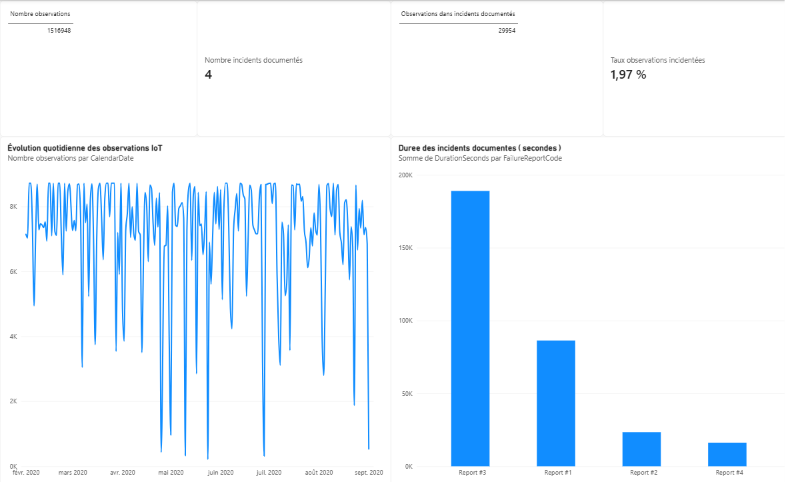
\includegraphics[width=\textwidth]{dashboard_1_vue_generale.png}
\caption{Page Power BI Vue générale}
\label{fig:dashboard1}
\sourcefigure{capture réelle présente dans reports/figures}
\end{figure}
La page comporte quatre cartes. Nombre observations affiche 1\,516\,948. Nombre incidents documentés affiche 4. Observations dans incidents documentés affiche 29\,954. Taux observations incidentées affiche 1,97\,\%. La courbe inférieure montre l'évolution quotidienne du nombre d'observations ; les creux visibles signalent une couverture quotidienne variable, et non nécessairement une panne. L'histogramme présente la durée des incidents documentés en secondes : le rapport 3 est le plus long, suivi des rapports 1, 2 et 4.

\section{Dashboard 2 -- Surveillance des capteurs}
\begin{figure}[H]
\centering
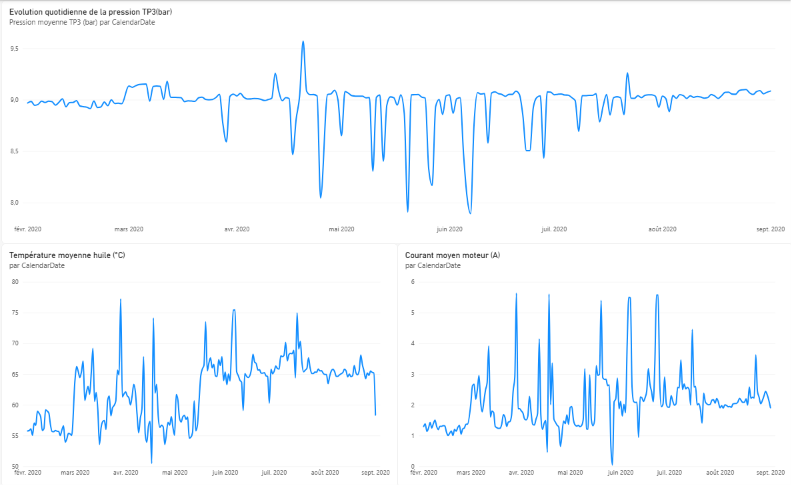
\includegraphics[width=\textwidth]{dashboard_2_surveillance_capteurs.png}
\caption{Page Power BI Surveillance des capteurs}
\label{fig:dashboard2}
\sourcefigure{capture réelle présente dans reports/figures}
\end{figure}
La page montre une courbe de la pression moyenne TP3, une courbe de température moyenne d'huile et une courbe de courant moyen du moteur. TP3 reste proche de 9 bar sur de nombreuses périodes mais présente des baisses ponctuelles jusqu'à environ 7,9 bar dans la visualisation. La température varie approximativement entre 53 et 77 degré C selon les dates affichées. Le courant présente une ligne de base autour de 1 à 3 A avec plusieurs pics visibles jusqu'à environ 5,6 A.

Ces amplitudes sont des lectures visuelles des axes du dashboard et ne constituent pas une nouvelle mesure calculée dans ce rapport. Un pic est un point à investiguer avec les autres signaux et le contexte de fonctionnement ; il ne prouve pas à lui seul une défaillance.

\section{Dashboard 3 -- Incidents et OLAP}
\begin{figure}[H]
\centering
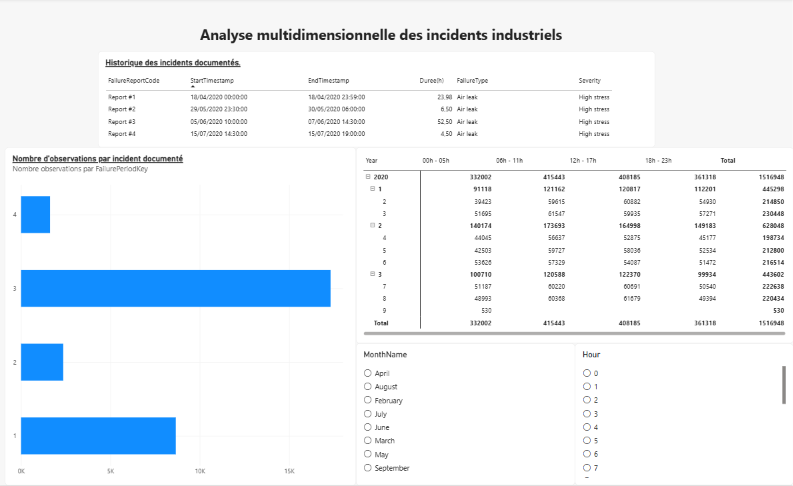
\includegraphics[width=\textwidth]{dashboard_3_incidents_olap.png}
\caption{Page Power BI Incidents et OLAP}
\label{fig:dashboard3}
\sourcefigure{capture réelle présente dans reports/figures}
\end{figure}
La page contient un historique tabulaire des quatre rapports, un histogramme du nombre d'observations par identifiant incident, une matrice temporelle et des segments MonthName et Hour. La table affiche Air leak et High stress pour les quatre lignes. Les durées visibles sont 23,98 h, 6,50 h, 52,50 h et 4,50 h, cohérentes avec les différences des bornes documentées.

La matrice présente Year en lignes et des tranches horaires en colonnes, avec un total général de 1\,516\,948. Cette structure illustre le pivot et le dice. Un utilisateur peut sélectionner un mois et une heure, puis observer le sous-ensemble correspondant. Le drill-down repose sur les niveaux de calendrier et doit conserver le contexte de filtre.

\section{Lecture OLAP}
Les trois pages couvrent les opérations suivantes :
\begin{itemize}
\item roll-up : passer des observations quotidiennes aux agrégats mensuels ;
\item drill-down : passer de Year à MonthName puis à CalendarDate ;
\item slice : sélectionner un seul FailureReportCode ;
\item dice : combiner un rapport avec MonthName et Hour ;
\item pivot : lire les heures en colonnes et les mois en lignes.
\end{itemize}
Power BI documente le drill comme une navigation dans une hiérarchie \cite{powerbiDrill}. Le projet doit cependant distinguer exploration OLAP et diagnostic : la visualisation organise les faits disponibles, elle ne remplace pas une expertise de maintenance.

\chapter{Analyse des résultats et discussion}

\section{Résultats observés}
Le modèle permet de répondre à quatre questions simples. Combien d'observations sont disponibles ? 1\,516\,948. Combien de périodes externes sont documentées ? quatre. Combien d'observations tombent dans leurs fenêtres inclusives ? 29\,954 selon la page Vue générale. Quelle est leur proportion parmi les observations ? 1,97\,\%.

Le comptage par rapport obtenu dans la table préparée est : 8\,657 observations pour le rapport 1, 2\,360 pour le rapport 2, 17\,315 pour le rapport 3 et 1\,622 pour le rapport 4. La somme vaut 29\,954. Cette cohérence valide la règle de rattachement appliquée au fait sans dupliquer FactFailurePeriod.

\section{Interprétation des capteurs}
Le dashboard de surveillance rend visibles trois familles. TP3 renseigne la pression du panneau pneumatique. Oil\_temperature renseigne la température de l'huile. Motor\_current renseigne l'effort électrique d'une phase. Les variations sont intéressantes pour une investigation car elles donnent un contexte conjoint. Cependant, le dataset ne fournit pas de seuil métier global validé par le projet ; le texte évite donc d'étiqueter une observation comme anormale sur la seule base d'un pic.

La courbe de couverture quotidienne présente des creux. L'audit explique que les intervalles supérieurs à la cadence modale sont fréquents. Un creux de nombre d'observations peut donc indiquer un trou d'acquisition ou une couverture variable. Il ne doit pas être interprété comme une durée d'arrêt du compresseur.

\section{Apport pour un responsable maintenance}
Un responsable peut utiliser la page générale pour vérifier le périmètre, la page capteurs pour sélectionner une période et la page incidents pour comparer un intervalle externe avec les observations correspondantes. Il peut aussi descendre de l'année au mois et à l'heure, ce qui facilite une question du type : quelles observations sont disponibles autour du rapport 3 ?

La valeur du modèle est la traçabilité. Chaque résultat est relié à un grain, une dimension temporelle, une mesure DAX et une règle d'association. Cette traçabilité rend les analyses révisables par un enseignant ou un ingénieur.

\section{Faits, interprétations et hypothèses}
\begin{table}[H]
\centering
\caption{Séparation des niveaux de preuve}
\label{tab:discussion}
\begin{tabularx}{\textwidth}{p{3.4cm}X}
\toprule
\textbf{Niveau} & \textbf{Exemple dans le projet}\\
\midrule
Résultat observé & Le dashboard affiche 1\,516\,948 observations et 4 incidents.\\
Interprétation technique & TP3, température et courant sont des axes pertinents pour une surveillance conditionnelle.\\
Hypothèse à vérifier & Une variation conjointe pourrait signaler un régime particulier ; elle nécessite une analyse métier.\\
Perspective & Ajouter des labels d'intervention et un modèle d'anomalie validé.\\
\bottomrule
\end{tabularx}
\end{table}

\section{Ce que le projet ne conclut pas}
Il ne calcule pas de disponibilité, de coût, de MTBF, de MTTR, de nombre d'interventions ou d'économie. Il ne classe pas toutes les observations hors fenêtre comme normales. Il ne déploie pas de Machine Learning de prédiction. Ces restrictions sont nécessaires pour respecter les données effectivement disponibles.

\chapter{Limites, perspectives et conclusion}

\section{Limites}
La première limite est temporelle : la cadence modale est de 10 secondes, mais la série comporte des irrégularités et des coupures. La deuxième est sémantique : les signaux numériques sont documentés, mais une règle unique de classification d'état n'a pas été validée. La troisième est événementielle : quatre rapports externes ne constituent pas une base complète des interventions. Enfin, le dataset ne contient pas les coûts, les ordres de travail, les stocks de pièces ou les temps d'immobilisation.

\section{Perspectives}
Une extension pourrait ajouter une table d'interventions validée, une dimension d'équipement si un parc est étudié, des règles de qualité de données automatisées, une agrégation contrôlée à cinq minutes et un système d'alertes. Une approche de détection d'anomalies pourrait ensuite apprendre un comportement de référence, mais elle devrait traiter les trous, les changements de régime et les fenêtres incidentes sans fuite d'information. Un modèle prédictif demanderait des données d'entraînement, un horizon, une fonction de coût et une évaluation temporelle.

\section{Conclusion générale}
Ce projet montre comment passer d'un historique de capteurs à un modèle décisionnel exploitable. La solution conserve le fait source, sépare les incidents externes, construit les dimensions temporelles et expose des mesures DAX simples. Les captures Power BI démontrent trois usages complémentaires : cadrer le périmètre, surveiller les signaux et explorer les incidents par OLAP.

La contribution principale n'est pas une promesse de prédiction automatique. Elle réside dans une préparation traçable, une modélisation cohérente et une lecture prudente des résultats. Cette base est suffisamment structurée pour accueillir ultérieurement des données de maintenance opérationnelle et évoluer vers un dispositif de maintenance conditionnelle puis prédictive.

\appendix
\chapter{Annexes techniques}

\section{Fichiers contrôlés}
\begin{tabularx}{\textwidth}{lX}
\toprule
\textbf{Artefact} & \textbf{Rôle}\\
\midrule
scripts/prepare\_powerbi\_data.py & Préparation reproductible des quatre tables.\\
powerquery/FactSensorObservation.pq & Import M et association temporelle.\\
powerquery/FactFailurePeriod.pq & Définition des quatre périodes externes.\\
powerquery/DimDate.pq & Dimension calendrier.\\
powerquery/DimTime.pq & Dimension seconde de la journée.\\
dax/measures.dax & Sept mesures DAX préparées.\\
powerbi/Smart\_Industrial\_Maintenance.pbix & Rapport Power BI inspecté.\\
\bottomrule
\end{tabularx}

\section{Relations Power BI}
\begin{enumerate}
\item DimDate[DateKey] vers FactSensorObservation[DateKey], active ;
\item DimTime[TimeKey] vers FactSensorObservation[TimeKey], active ;
\item DimDate[DateKey] vers FactFailurePeriod[StartDateKey], active ;
\item DimDate[DateKey] vers FactFailurePeriod[EndDateKey], inactive.
\end{enumerate}
Les filtres sont à sens unique des dimensions vers les faits. Aucune relation directe entre les deux faits n'est requise.

\section{Validation de compilation}
Le dossier est organisé pour une compilation pdfLaTeX avec Biber. La validation finale a été effectuée avec MiKTeX 26.5 en appelant directement ses exécutables locaux, sans modifier le PATH Windows. Le PDF final contient 41 pages physiques : 32 pages sont numérotées dans le corps du rapport, les pages restantes correspondant aux éléments liminaires et aux pages non numérotées selon le template. La table des matières, les références, les figures et la pagination ont été régénérées après l'intégration des trois captures Power BI. Les avertissements restants sont non bloquants et limités à la composition de certains tableaux et à un repli de police.

\section{Limite de résolution des dashboards}
Les trois captures disponibles sont des images raster d'environ 785 à 793 pixels de largeur. Les originaux HD n'étant pas présents dans le dépôt, aucune interpolation artificielle n'a été appliquée. La reprise manuelle recommandée consiste à exporter les trois pages depuis Power BI Desktop en haute résolution, puis à remplacer les fichiers de figures en conservant les proportions et les légendes existantes.

\backmatter
\printbibliography[heading=bibintoc,title={Bibliographie et webographie}]
\end{document}
